\documentclass[tikz,border=10pt]{standalone}
\usetikzlibrary{matrix,positioning,quotes,fit}
\usetikzlibrary{backgrounds}
\tikzset{standard/.style={matrix of nodes,left delimiter={(},right delimiter={)},inner sep=0pt,nodes={inner sep=0.3em}}}
\tikzset{submatrix/.style = {rectangle, rounded corners,
  fill=yellow, draw, inner sep=0pt}}
\begin{document}
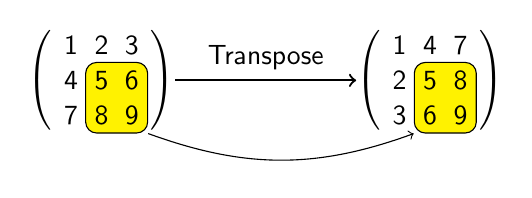
\begin{tikzpicture}[every node/.append style={font=\sffamily}]
  \matrix[standard] (m)  {
       1 & 2 & 3 \\
       4 & 5 & 6 \\
       7 & 8 & 9 \\};
  \matrix[standard,right = 3cm of m] (n) {
       1 & 4 & 7 \\
       2 & 5 & 8 \\
       3 & 6 & 9 \\};
  \draw[->,shorten <=1em,shorten >=1em,thick] (m.east) to["Transpose"] (n);
 \begin{scope}[on background layer]
   \node (m1) [submatrix, fit=(m-2-2) (m-3-3)] {};
   \node (n1) [submatrix, fit=(n-2-2) (n-3-3)] {};
 \end{scope}
 \draw [->] (m1.south east) to[bend right=20] (n1.south west);
\end{tikzpicture}
\end{document}
